\documentclass{article}
\usepackage{geometry}
\usepackage{amsmath}
\usepackage{amsfonts}
\usepackage[square, comma, sort&compress,numbers]{natbib} 
\usepackage[usenames, dvipsnames]{color}
\usepackage{graphicx}
\usepackage{caption}
\usepackage{subcaption}
\usepackage[normalem]{ulem}
\useunder{\uline}{\ul}{}
\newcommand{\specialcell}[2][c]{%
  \begin{tabular}[#1]{@{}c@{}}#2\end{tabular}}

\begin{document}

\begin{titlepage}
    \begin{center}
        \vspace*{1cm}
        
        \textbf{Building personalized summaries from movie reviews}
        
        \vspace{0.5cm}
       
        \vspace{1.5cm}
        
        \textbf{Sara El Aouad}
        
        \vfill
        
       
        \vspace{0.8cm}
       
        Academic advisor: Renata Teixeira, Vassilis Christophides\\
        Industrial Advisors: Patrick Perez, Christophe Diot\\
        
        10/02/2017
        
    \end{center}
\end{titlepage}
\newpage

Many moviegoers enter detailed reviews of movies they have watched on sites such as IMDB and Rotten Tomatoes. The corpus of online reviews represents a source of rich meta-data for each movie.
%Our goal is to leverage this plethora of information in order to. 
The challenge we face is to mine the noisy free-text reviews from a heterogeneous set of people to understand than extract meaningful summaries of movie reviews. We are tackling this challenge in five steps. First, we collected our data by crawling the IMDB website as it has movies metadata like the movie genre and the year of appearance, it also has the movie list of reviews. The outcome of this step is a raw dataset of movies, users and reviews. Second, we analyzed this dataset in order to understand its characteristics as the algorithms we would like to use will heavily depend on our dataset. Third as shown in figure \ref{introChapter1} we have pre-processed the textual reviews to remove the noisy words and to standardize the data , the outcome of this step serves as in input to the fourth step which is representing words in a vector space. In the fifth and last step we introduce the similarity metrics we use in order to compute the similarity between two vectors and set of vectors.
\section{Dataset}
\label{section:dataset}
In this section we first start by describing the dataset used in this thesis along with the basic notations we will use to describe our dataset. 
\subsection{Dataset characteristics}
For this thesis we crawl the \textit{IMDB} website in the period of (). We chose this data to build and evaluate our algorithms because in addition to the overall rating that users give to a movie, they also provide a textual review to explain their opinion. As shown in Figure \ref{umlDiagram}, this dataset contains three different entities the Movie entity that has four different attributes: the movie unique identifier i.e. the \textit{movieId} the movie title, the year of appearance of the movie  and the list of the IMDB genres for example [Romance, Comedy]. For the User entity we only have the user unique identifier as an attribute. Finally we have the Review entity that has three attributes, three attributes, the review Id which is the (movieId, userId)tuple because a user can only write one review per movie, the second attribute is the text review which is the actual review that the user has written about the movie. The final review entity attribute is the rating given by the user to the movie ranging from 1 star to 10 stars. It's worth noting that a user might write a review along with a rating or just a review orgive a rating. In our dataset we have 9888 movies  and 763571 reviews; the details are illustrated in Table \ref{datastat}.

As shown in Figures \ref{NbReviewsPerMovie} and \ref{NbRatingsPerMovie} the median number of reviews is 39 review and the median number of ratings is 31 per movie. We can conclude that our dataset is somewhat sparse.
To overcome this issue we have splitted the dataset into three categories, according to the movies number of reviews. The three categories we propose are the following : \textbf{off-off Broadway movies}, these movie have a low number of reviews: less than 20 reviews, these movies constitute 20\% of the total number of movies. The second category is the \textbf{Popular movies} category, in this category the movies have a number of reviews between 20 and 110 reviews, 40\% of the total number of movies are popular movies. The final category is the \textbf{Blockbuster movies} category, these movies have a very high number of reviews (movies having more than 110 reviews) for example the movie ``Inception" with 820 textual reviews,  20\% of movies in our dataset are Blockbuster movies.
We would like to evaluate the performance of our summarization algorithm for this three different movie categories.


Since we want to profile users using their past textual reviews and the ratings they have given to movies, it is essential to analyze how much data we have about each user. Figure \ref{NbReviewsPerUser} and Figure \ref{NbRatingsPerUser} show the distribution of the number of reviews and ratings given by users respectively. We could observe that there is a high variety of the number of reviews and ratings given by users. 

In addition to data sparseness, another issue of great concern is the review length. Usually natural language processing/machine learning techniques work better with longer text. To this end, we did similar analysis to the text lengths of the reviews. It turned out that the reviews are of decent length generally: the the median length on all the reviews is 231 words. Figure \ref{NbWordsPerReview} further confirms that. In order to create our vocabulary set we have built a corpus of textual reviews which is the concatenation of all the movie reviews written by all users.
We did a similar analysis for the sentences length, in Figure \ref{NbWordsPerSentence} we can see that in 60\% of the cases, the sentences length  is bigger than 10 words per sentence, which means that the sentences are usually long and complex therefore harder to analyze. For the 1\% left  sentences with more than 50 words is due to some badly written sentences where users did not use properly the punctuation. 

\begin{table}[]
\centering
\caption{Dataset statistics}
\label{datastat}
\begin{tabular}{|l|l|l|l|l|}
\hline
\#of movies & \#of users & \#of reviews & \#of ratings & \#of sentences \\ \hline
9887        & 17131      & 763571       & 775654       & 11437314       \\ \hline
\end{tabular}
\end{table}
\subsection{Problem statement}
We have a set of movie $M = \{m_{1},...,m_{l}\}$ each movie has a set of reviews  $R_{m} = \{r_{m1},..., r_{mq} \}$ each review contains a set of sentences $S_{r} = \{s_{r1},..., s_{rp} \}$ and each sentence contains a set of words $s_{r} = \{w_{r1},..., w_{rq} \}$.
The vocabulary set is the concatenation of all the words of all the sentences reviews.
Given a set of domain knowledge aspects $A = \{a_{1},..., a_{f} \}$, our goal is to detect from our vocabulary for each aspect the distinctive related terms to it while allowing overlap between the terms of each aspect.
\subsection{Basic notations}
In our dataset we have a set of reviews $R = \{r_{1},..., r_{q} \}$ regarding a set of movies $M = \{m_{1},...,m_{l}\}$. Each review contains a set of sentences. We denote the sentences of all reviews as  $S = \{s_1, ..., s_m\}$ where $m$ is the total number of sentences. As described in subsection \ref{subsection:preprocessing} each sentence is tokenized then lemmatized so we end up with a set of unique words $V= \{w_{1},..., w_{n} \}$, $n$ being the size of the vocabulary. The goal of words representation is to create a word representation matrix 
$W$ $\in$  $\mathbb{R}^{d*n} $
where $d$ is the vector dimension whereas $n$ is the size of the vocabulary.
Such representation allow us to map each word $w$ to its word vector representation $\vec{v}$.
\section{Vocabulary}
\label{vocab}
Our crawled corpus of reviews contains lots of noise that can cause misleading results while representing words as vectors such as punctuation, html tags and urls. These issues can be solved by using natural language techniques which are called text pre-processing. The output of this step serves as the vocabulary that will be used while representing words as vectors.
\begin{figure}
 \begin{center}
 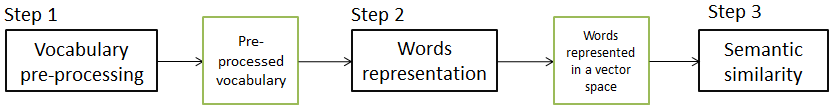
\includegraphics[scale=0.6]{introChapter1} 
 \caption{ Overview of the system} 
  \label{introChapter1}
  \end{center}
 \end{figure}
 
\begin{figure}
 \begin{center}
 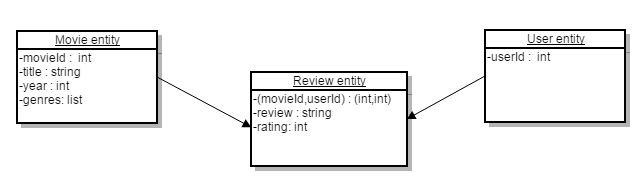
\includegraphics[scale=0.6]{uml.png} 
 \caption{Different dataset entities} 
  \label{umlDiagram}
  \end{center}
 \end{figure}
\label{subsection:text preprocessing}
\vspace{1.5mm}\noindent \textbf{Words tokenization} \\
Given a document, tokenization is the task of splitting it into  small pieces, called \textit{tokens} or \textit{lemmas}, perhaps at the same time as removing certain characters, such as punctuation. 
Here is an example of tokenization: 'This was a good movie!' the output would be ['this', 'was', 'a', 'good', 'movie'].
We use the Penn Treebank Tokenizer implemented in the  natural language NLTK for words tokenization \cite{nltk:2006, nltk:2009}.\\
\vspace{1.5mm}\noindent \textbf{Words lemmatization}\\
Documents usually use different forms of the same word for example drive driving driven depending on the context.
The goal of lemmatization is to reduce inflectional forms  of a word to a common base form. For instance: the verb 'driving' might become 'drive'. 
We use the WordNet lemmatization algorithm as implemented in NLTK \cite{nltk:2006, nltk:2009} as a second preprocessing step.\\
\vspace{1.5mm}\noindent \textbf{Collocation detection}\\
A collocation or a compound expression is defined as a sequence of words that together mean a new word, for example ``science fiction" or ``chick flick". Even if flick is a synonym of movie, it's unconventional to find ``chick movie".
Thus it is important to detect these compound expressions and replace them in the whole corpus before combining synonyms.
Each found collocation is replaced in the whole corpus as a single word, for example ``chick flick" is replaced by ``chick-flick" for each of its occurrences in the Dataset.
In order to find these collocations we use a statistical measure, which is defined as follows:

$$score(w_{1},w_{2})= \frac{p(w_{1},w_{2})}{p(w_{1})p(w_{2})}$$

 where $w_{1}$ and $w_{1}$ denote two different words in the corpus that we want to measure the score of.  $p(w_{1},w_{2})$ is the probability of the bigram $(w_{1},w_{2})$ in the corpus and $p(w_{1})$ and $p(w_{2})$ are respectively the probabilities of $w_{1}$ and $w_{1}$ in the corpus.
For each tuple in our dataset we calculate its score, and we combine just the words having a score above 9. This threshold was determined empirically.

\begin{figure}
\centering
\begin{minipage}{.6\textwidth}
  
  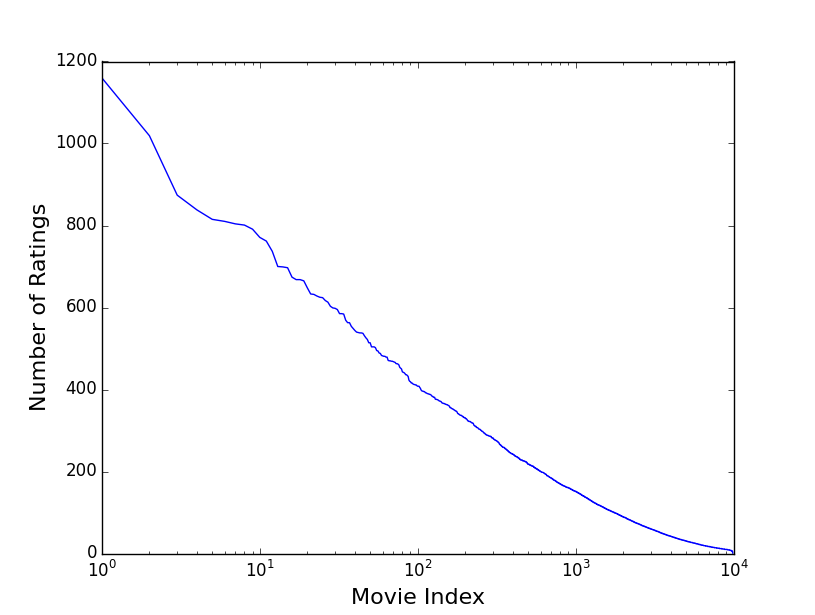
\includegraphics[width=\linewidth]{NbRatingsPerMovie.png}
  
  \captionof{figure}{Distribution of the number\\ of ratings per movie}
	 \label{NbRatingsPerMovie}
\end{minipage}%
\centering
\begin{minipage}{.6\textwidth}
  
  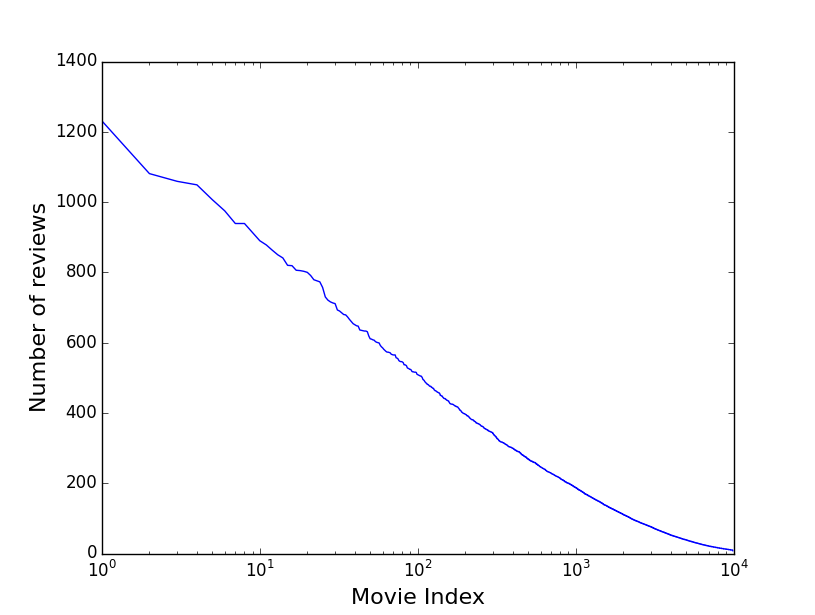
\includegraphics[width=\linewidth]{NbReviewsPerMovie.png}
  \captionof{figure}{Distribution of the number \\ of reviews per movie}
  \label{NbReviewsPerMovie}
\end{minipage}
\end{figure}

\begin{figure}
\centering
\begin{minipage}{.6\textwidth}
  
  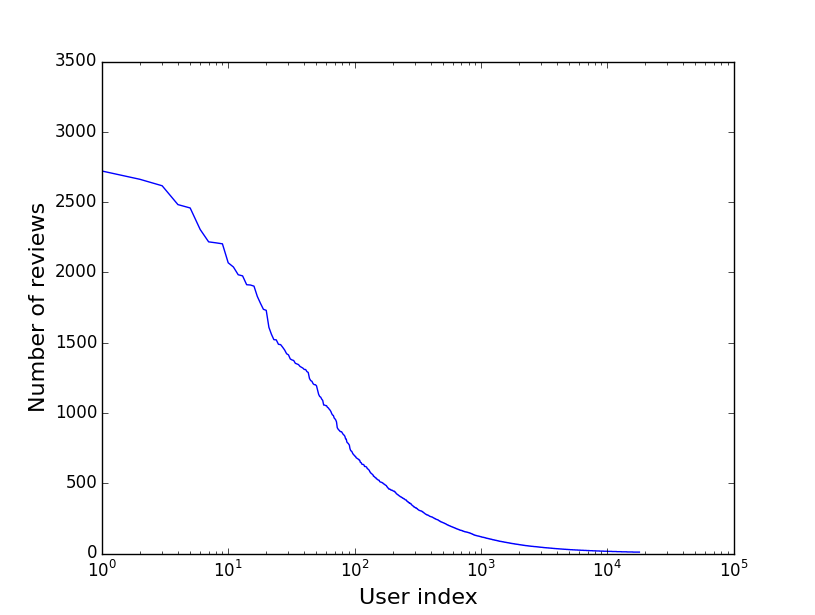
\includegraphics[width=\linewidth]{NbRatingsPerUser.png}
  
  \captionof{figure}{Distribution of the number\\ of ratings per user }
	 \label{NbRatingsPerUser}
\end{minipage}%
\centering
\begin{minipage}{.6\textwidth}
  
  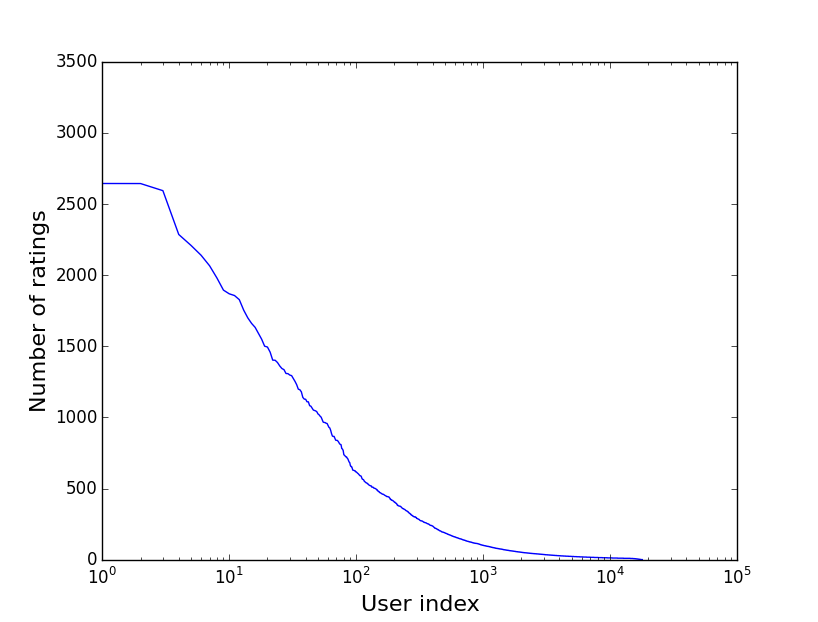
\includegraphics[width=\linewidth]{NbReviewsPerUser.png}
  \caption{Distribution of the number\\ of reviews per user} 
  \label{NbReviewsPerUser}
\end{minipage}
\end{figure}

\begin{figure}
\centering
\begin{minipage}{.6\textwidth}
  
  \includegraphics[width=\linewidth]{NbOfWordsPerReview.png} 
 \caption{Distribution of the number of words per review} 
  \label{NbWordsPerReview}
\end{minipage}%
\centering
\begin{minipage}{.6\textwidth}
  
  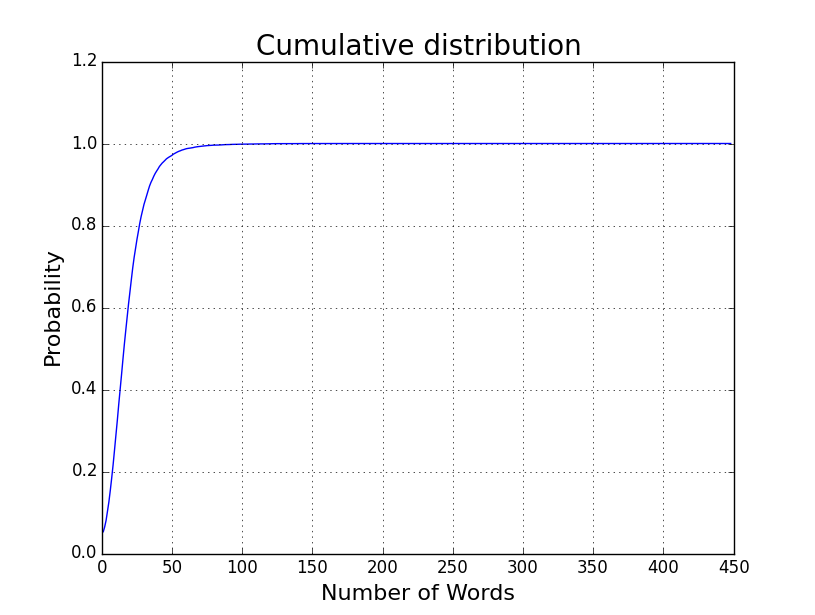
\includegraphics[width=\linewidth]{NbOfWordsPerSentences.png}
  \caption{CDF of the number of words per sentence} 
  \label{NbOfWordsPerSentences}
\end{minipage}
\end{figure}



\section{Words representation}
After pre-processing the corpus of reviews and creating our vocabulary the next step is to represent words in a vector space in order to be able to compute the similarity between words.
In this section we first introduce the different approaches of representing words in a vector space from the literature then we present then we briefly introduce the approach we are using for this thesis.

\subsection{Background}

The distributional hypothesis by Harris states that words with similar meaning occur in similar contexts \cite{harris:1954}. This
implies that the meaning of a word can be inferred from its distribution across contexts. The goal of distributional semantics
is to find a representation, e.g. a vector, that encodes the semantic of the word.
The general idea behind representing words as vectors is to use distributional statistics to generate high-dimensional vector
spaces, where a word is represented by a vector that encodes its semantic.

\subsubsection{Word Count/context matrix}
The traditional way to represent words in a vector space is to construct a high dimensional sparse matrix $M$, where each row represents a word $w$ in the vocabulary $V$ and each column is a word context $c$. The value
of each matrix cell $M_{ij}$ measures how often	a word	$w_{i}$ occurs with the context $c_{j}$. A popular measure of this association is pointwise mutual information (PMI) from Church et al. \cite{church:1989}. PMI is defined as a measure of association between two words that tells us how much more often than chance the two words co-occur together. Formally to compute the PMI score between a word $w$ and a context word $c$ we use the following formula \cite{church:1989}:
$$PMI(w,c)=log_{2} \frac{p(w,c)}{p(w).p(c)}$$
$p(w,c)$ is the probability of the bigram $(w,c)$ in the corpus and $p(w)$ and $p(c)$ are respectively the probabilities of $w$ and $c$ in the corpus.
PMI values range from negative to positive infinity. But negative PMI values(which means that words are co-occurring less often than we would expect by chance) tend to be unreliable unless the dataset used is huge. The Matrix M is also ill-defined, for example a word context pair $(w,c)$ that never co-occurred together will have a value of 0, while a word context pair that rarely co-occurred together will have a negative value, which is inconsistent.
A more consistent approach is to use positive PMI (PPMI), in which all negative values are replaced by 0:
$$PPMI(w,c)= max(log_{2} \frac{p(w,c)}{p(w).p(c)},0)$$
A well-known shortcoming of PMI, and also PPMI, is its bias towards infrequent events  \cite{turney:2010}. A rare context $c$ that co-occurred with a target word $w$ even once will often yield relatively high PMI score because of the very small value of $P(c)$ in the PMI's denominator. This leads to having high scores for context words  that rarely co-occur with $w$. Nevertheless, the PPMI measure is widely considered as state-of-the-art for these kinds of distributional-similarity models.
Using such a high dimensional space leads to having very sparse vector representations that comes from data scarcity. One way of dealing with this problem is to use a dense low-dimensional vector representation.
Such vectors can be obtained by performing dimensionality reduction over the sparse high-dimensional matrix.
A common method of doing so is truncated Singular Value Decomposition (SVD) \cite{svd:1936}, which finds the optimal rank $k$ factorization. It was popularized in NLP via Latent Semantic Analysis (LSA) \cite{lsa:1990}. LSA has been proved by Turney et al.  \cite{turney:2001} to give better results with relatively little text.
\subsubsection{Words representations from prediction}
A second method for generating word representation is inspired from the neural network models used for language modeling. Traditionally neural network language models are given a word and predict context words. This
prediction process can be used to learn representation for each word. The intuition is that words with similar meanings often occur near each other in texts. 
When trained on a textual corpus, the neural models learn the words representations by starting with a random vector and
then iteratively shifting a word's representation to be more like the representation of neighboring words, and less like the representations of words that don't occur nearby.

The development of models of embeddings is an active research area, with new models including GloVe \cite{glove:2014} (based on ratios of probabilities from the word-word co-occurrence matrix), the word2vec tool \cite{mikolov:2013} that implements  the continuous bag-of-words and skip-gram architectures for computing vector representations of words or the recently introduced sparse embeddings based on nonnegative matrix factorization \cite{fyshe:2015}.

In our work we use the recent findings in the distributional semantics areas which is the prediction models in order to infer the words embeddings because they are faster to train  \cite{levy:2015, mikolov:2013}. They have also been proven to give very good results for different prediction tasks  \cite{ collobert:2011, fyshe:2015}.

\subsection{Word2vec}
Here we describe the word embedding tool we use (word2vec), we first start by introducing the two different models used in word2vec and we also explain the different parameters implemented in word2vec .
After explaining how we represent words in a vector-space we formally define how we compute the similarity between vectors than between two sets of vectors.

\begin{figure}
 \begin{center}
 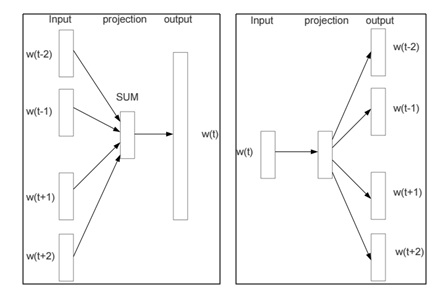
\includegraphics[scale=0.6]{w2vecModels.png} 
 \caption{ The CBOW model predicts the current word based on the
context (image on the left), and the Skip-gram predicts surrounding words given the current word (image on the right). } 
  \label{word2vecmodels}
  \end{center}
 \end{figure}
%Here we describe the word embedding technique we use (word2vec) although many word embeddings models could be used \cite{glove:2014}.
 
\subsection{Word2vec models}
Word2vec introduced by Mikolov et al. \cite{mikolov:2013}, is one of the most popular techniques for learning a word embedding over billions of words. When trained on a corpus, Word2Vec learns for each word its representation in a low-dimensional vector space. Words that are used and occur in the same contexts in the original corpus tend to have similar meaning and are mapped to nearby points in this low-dimensional space. We choose Word2Vec model in our work, because it has a number of desired properties for our problem. First it's completely unsupervised, which means that we can learn the representation of the words directly from our corpus without the need of a training dataset that requires manual annotation which is expensive and requires
an extensive human effort especially on large datasets. Second it's efficient to train, the word2vec model is  fast to train even on large datasets. 
Third the similarity between words is dependent on the movie reviews context, for example using a general thesauri will give as a synonym for the word ``picture" the word ``photograph", whereas in the context of movies the word ``picture" is synonymous of the word ``movie".
In the original paper(Mikolov et al. \cite{mikolov:2013} the authors introduced two distinct model the continous bag of words model denoted CBOW and the skip gram model. 
As shown in Figure \ref{word2vecmodels} the skip gram model predicts the surrounding words given the center words, whereas  the continuous bag of words model (CBOW) predicts the neighboring words given the center word.
Algorithmically, the Continuous Bag-of-Words model (CBOW) and the Skip-Gram model are similar, except that CBOW predicts target words (e.g. ``movie") from source context words (``you must go and see this"), while the skip-gram does the inverse and predicts  context-words from the target words. This inversion has the effect that CBOW smoothes over a lot of distributional information (by treating an entire context as one observation). This makes the CBOW model useful for smaller datasets and also faster to train than the skip-gram model. However, skip-gram treats each context-target pair as a new observation, and this tends to do better when we have larger datasets it also represents well even rare words or phrases. 
While CBOW and skip-gram are similar algorithms and produce similar embeddings, it has been shown that the skip-gram model gives better results than the CBOW model \cite{mikolov:2013} this is why we are going to use the skrip gram model for our work.
In the next sub section we explain the skip gram model.
\subsubsection{The Skip gram model}  
The skip-gram embedding model  seeks to represent each word $w \in V_{w}$ and each context $c \in V_{c}$ as a  d-dimensional vectors $\vec{w}$ and $\vec{c}$, such that words that are “similar” to each other will have similar vector representations.
It does so by trying to maximize the likelihood of the prediction of contextual words given the center word. More formally
let's consider that we have corpus of length $T$, and let's consider the tieth word word $w^{t}$, whose index in the vocabulary is $j$, so we'll call it $w_{j}$  $(  j \in |V|)$. The skip-gram model predicts each neighboring word in a context window of size $2*L$ words, ($L$ being the size of the window)  from the current word. So for a context window
$L = 2$ the context is $[w^{t-2}, w^{t-1}, w^{t+1}, w^{t+2}] $ and we are predicting each of these  words from word $w_{j}$. Let's assume that we are predicting one of the $2L$ context words, for example $w^{t+1}$, whose index in the vocabulary is $k$ ( $k \in  |V|$). Computing the probability $p(w_{k}|w_{j})$ is computing the dot product between the vectors of the context vector for $w_{k}$ and denoted $\vec{c_{k}}$ and  the vector for $w_{j}$ denoted $\vec{v_{j}}$. The dot product of $\vec{c_{k}}$ and $\vec{v_{j}}$ is not a probability, it's just a number ranging from -$\infty$ to +$\infty$. As mentioned in \cite{mikolov:2013} The softmax function is than used  to normalize the dot product into probabilities. Computing this denominator requires computing the dot product between each other word $w$ in the vocabulary with the target word $w_{i}$.

$$ p(w_{k}|w_{j})=\frac{exp(c_{k},v_{j})}{ \sum_{i \in |V| }exp(c_{k},v_{i}) }$$
%equation

%\subsubsection{The CBOW model}
%The CBOW (continuous bag of words) model is roughly the mirror image of the skip-gram model. Like skip-grams, it is based on a %predictive model, but this time predicting the current word wt from the context window of words around it.




\subsection{Word2Vec Parameters Setting}
\subsubsection{Dynamic window size}
The common way of defining a window context is usually using a constant-sized unweighted context window. For instance, if the window size is 5, then a word five tokens apart from target will have the same weight same as the adjacent word.
Following the intuition that contexts closer to the target are more important, context words can be weighted according to their distance from the target word. Word2vec uses a similar schema for weighting the context words. In our dataset we use a context window size of 10 as in \cite{mikolov:2013}, because it was proven that taking a window bigger than 5 gave a higher accuracy. this window size was also tuned for our dataset using visual inspection.  \\
\subsubsection{Sub-Sampling}
Subsampling is a method of damping the effect of  very frequent words, this has also the effect of removing stop-words. The subsampling method presented in Mikolov et al. \cite{mikolov:2013} randomly removes words that are more frequent than some threshold t with a probability of p, where f represents the word’s corpus frequency:
$$ p=1-\sqrt{\frac{t}{f}} $$
Following the recommendation in Mikolov et al. \cite{mikolov:2013}, we use $t = 10^{-5}$in our experiments.
In word2vec is that the removal of tokens is done before the corpus is processed into (word,context)
pairs. This has the effect of enlarging the context window size for many tokens, because they can now reach words that were not in their original window size.
It was also reported in \cite{mikolov:2013} that the subsampling of the frequent words improves the training speed several times and makes the word representations significantly more accurate.
\subsubsection{Rare words delation}
While it is common to ignore words that are rare in the training corpus, word2vec removes these tokens from the corpus before creating context windows. As with subsampling, this variation narrows the distance between tokens, inserting new word-context
pairs that did not exist in the original corpus with the same window size. In our work we set the threshold for deleting word to 10.


\subsection{Word2vec examples}
In order to measure the similarity of words, the first information we need is a measure of distance: words that are closer in distance tends to be more similar. Ideally such distance should capture semantic closeness. As mentioned earlier we use the Word2Vec tool that is based on the idea that two words are more similar if they tend to appear in the same context. Given an unlabeled training corpus, the Word2Vec skip-gram model produces a vector for each word in the corpus that encodes its semantic information. 
 


\begin{figure}
 \begin{center}
 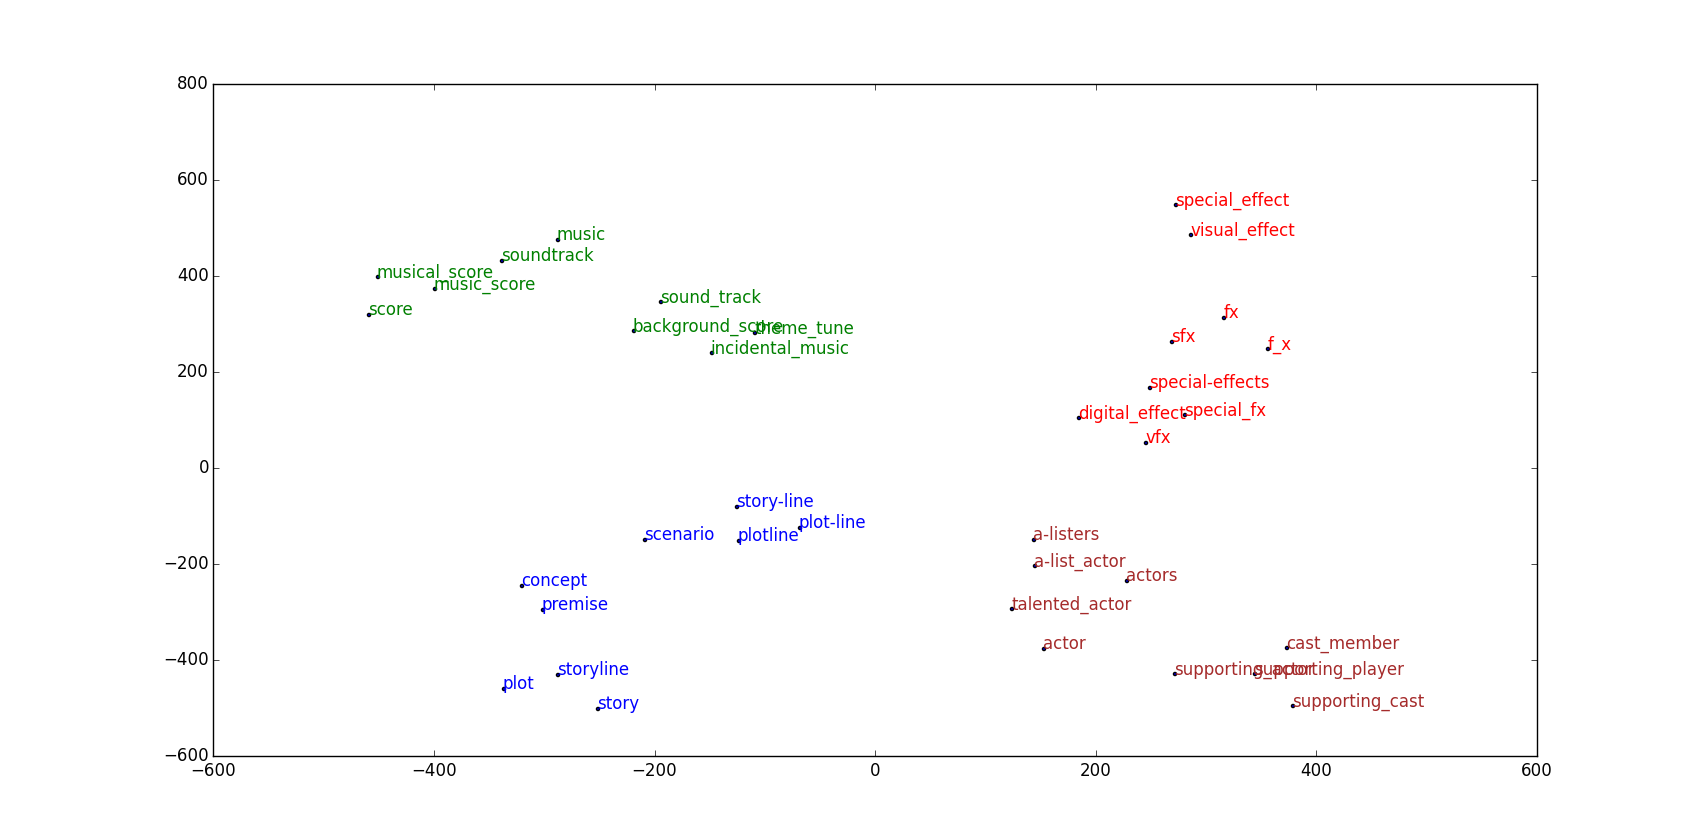
\includegraphics[scale=0.3]{tsne_clusters2.png} 
 \caption{Clusters of semantically similar words emerge when the
word2vec vectors are projected down to 2D using t-SNE. } 
  \label{w2vecclusters}
  \end{center}
 \end{figure}


We train the Word2Vec on our processed vocabulary that we described in section \ref{section:vocab} to generate the words representations. In figure \ref{w2vecclusters}  we can see that words that are semantically similar are close to each other and that words that are similar end up being clustered nearby each other. For example the cluster in red is about ``visual-effect", whereas the cluster in blue is about word that are semantically similar to the word ``story".
Before visualizing the words into the 2 dimensional space we use a dimensionality reduction step where word vectors are projected down to 2D vector space. We use the t-distributed Stochastic Neighbour Embedding (t-SNE) which is a dimensionality reduction technique that helps to visualize large real-world datasets with limited computational demands. T-SNE is well-suited for high-dimensional data that lies on several different, but related, low-dimensional vector space dimensions \cite{tsne:2008}. It has also been in \cite{tsne:2008} proven that t-sne gives better results than the traditional dimensionality reduction techniques such as PCA \cite{pca:1987} or SVD \cite{svd:1936}.




\begin{table}[]
\centering
\caption{Examples of the closest words to a given word using the Word2Vec model.}
\label{wordvec}
\begin{tabular}{|c|c|c|}
\hline
good&funny&kid\\
\hline
decent  0.73&hilarious  0.75&boy  0.75\\
great  0.7&amusing  0.71&teenager  0.68\\
fine  0.67&humorous  0.69&girl  0.64\\
nice  0.65&laugh-out-loud  0.66&lad  0.6\\
bad  0.63&scary  0.63&youngster  0.57\\
solid  0.62&clever  0.6&child  0.56\\
terrific  0.59&comical  0.58&brat  0.56\\
fantastic  0.55&witty  0.56&guy  0.53\\
wonderful  0.54&touching  0.56&man  0.52\\
competent  0.53&entertaining  0.53&bully  0.52\\
\hline
\end{tabular}
\end{table}


%Another problem that we can detect is that the closest similar word to science is fiction, while we know that science fiction is a compound expression. An explanation for such word similarity between this type of relatedness is that naturally they co-occurr in the same contexts. 
%The second limitation of this model is that even in related words we can find different kinds of relatedness. Hypernemy

\section{Semantic similarity}
The output of the last section is the representation of each word as a vector, the goal of this section is to use the words representation which are the vectors for vectors similarity computation. 
In our setting we have three different use cases. In the first use case we want to find the related words to a particular word. For this we would like to have a similarity metric between two vectors.
In the second use case the first set of vectors $X$  contains a set of word vectors that are similar to each other and that represent the same concept. Whereas $Y$ is set of word vectors that constitutes a sentence. We call this similarity metric the ``Closest pairs distance". 
In the third use case we want to compare between two sets of vectors $X$ and $Y$, given that the words in  $X$ and $Y$ are not necessarily similar to each other. This similarity metric is used when computing the similarity between two different sentences and is called the ``Word Movers Distance" (WMD).
We first define the similarity metric used to compute the similarity between two vectors then we introduce suitable metrics for computing the similarity between two sets of vectors.
\subsection{Similarity Metrics on Vectors}
To define the similarity between two target words $x$ and $y$, we need a measure for taking two such vectors and giving a measure of vector similarity. By far the most common similarity metric is the cosine of the angle between the vectors \cite{manning:1999}. The cosine—like most measures for vector similarity used in NLP is based on dot product. The dot product acts as a similarity metric because it will tend to be high just when the two vectors have large values in the same dimensions.
The dot product is higher if a vector is longer, with higher values in each dimension. The simplest way to solve this problem is to normalize the dot product by dividing it by the lengths of each of the two vectors which is the cosine measure.
To compute the similarity of two word vectors $\vec{x}$ and $\vec{y}$ we use the following formula:

$$cosine(\vec{x}, \vec{y})=\frac{\vec{x}. \vec{y}}{|\vec{x}| |\vec{y}|}= \frac{\sum_{i}^{n} x_{i}y_{i}}{\sqrt{\sum_{i}^{n}x_{i}^2} \sqrt{\sum_{i}^{n} y_{i}^2}}$$
The cosine value ranges from 1 for vectors pointing in the same direction, through 0 for vectors that are orthogonal, to -1 for vectors pointing in opposite directions.
The Table \ref{wordvec} shows the ten words having embeddings closest to a given word, the scores represent the cosine similarity score between each two word vectors.
As we can see from Table \ref{wordvec}, the similarity scores are able to illustrate the semantic relationship between two words, for example ``great" is a synonym of ``good" and ``amusing" is  synonym of ``funny". But the first limitation of this type of word representation is that it assigns a high degree of similarity to antonyms as well as synonyms. Words having a high cosine similarity score are typically semantically related, which includes synonyms, antonyms and different kinds of semantic relationship, as they often co-occur in similar contexts. As we can conclude from the results ``bad" is antonym of ``good", even though it has the highest similarity score compared to other words. This problem only happens with adjectives, we don't have similar problems with noun words.
\subsection{Similarity Metrics on Vector Sets}
\begin{figure}
 \begin{center}
 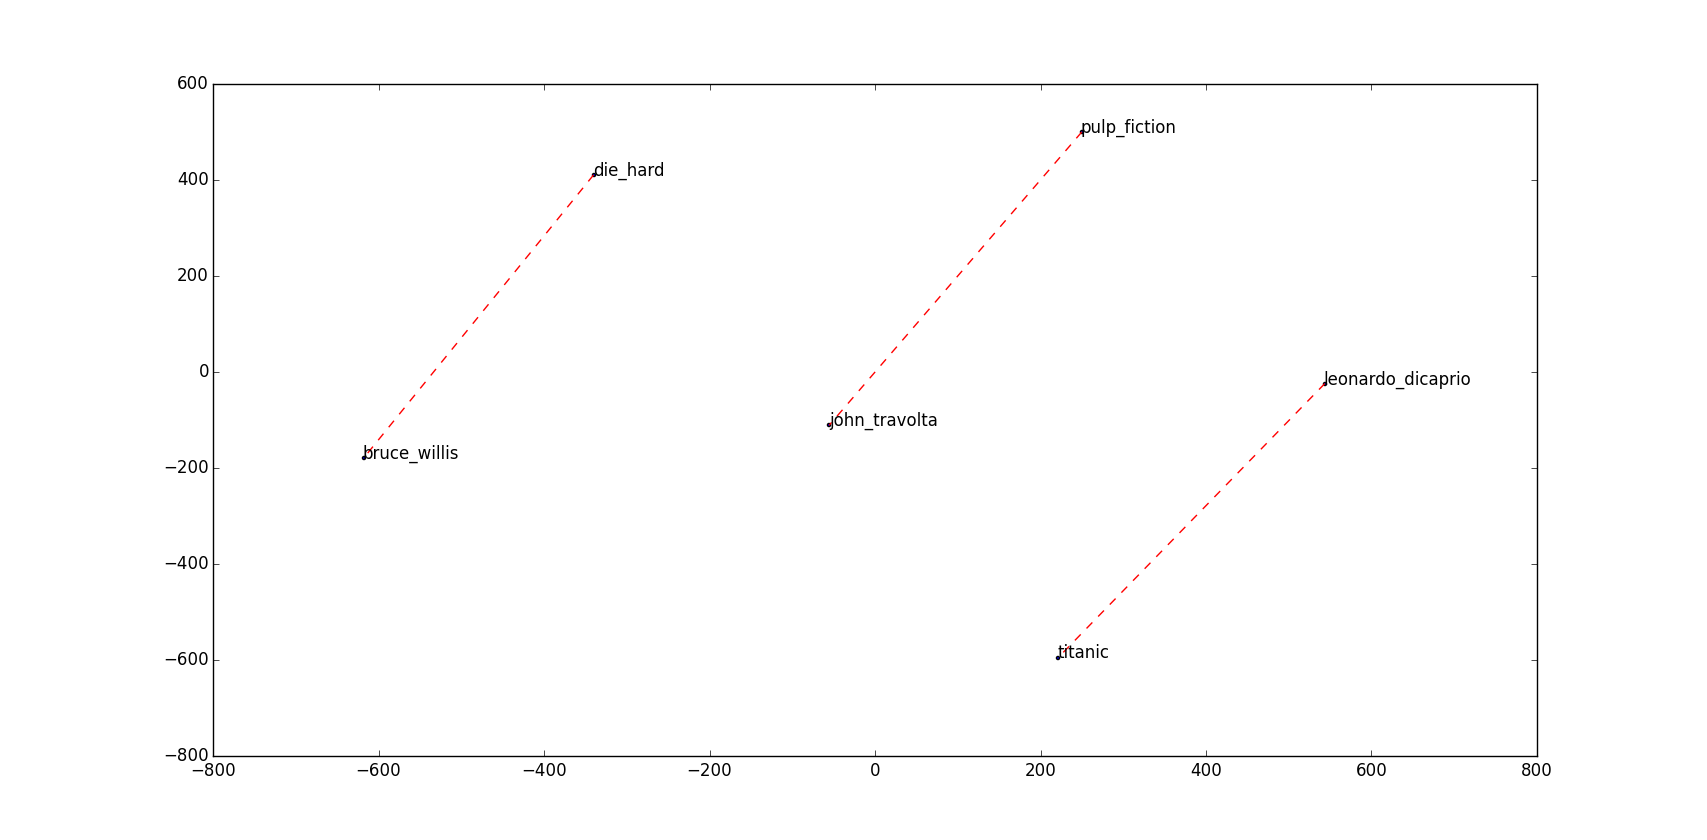
\includegraphics[scale=0.3]{tsne_analogies2.png} 
 \caption{ Analogy task (main-actor:movie) based on word2vec vectors  } 
  \label{analogytask}
  \end{center}
 \end{figure}
In this section we introduce the different distance measures that we are using during this work. As described in the previous sections each word is represented by its vector representation.
Let us assume that we want to measure the similarity between two sets of vectors X and Y. Where 
$X=\left \{ x_{1}, ... , x_{n} \right \}$ and $Y= \left \{ y_{1}, ... , y_{m} \right \}$,  $n$ and $m$ being respectively the sizes of $X$ and $Y$.
We can compare two vectors by computing the cosine similarity between their corresponding vectors. This measures the similarity between two vectors rather well \cite{manning:1999}. But, what would be a suitable distance for comparing two sets of vectors? 

We explain both similarity metrics ``Closest pairs distance" and ``Word movers distance" in the following sub-sections. 
\subsubsection{Closest pairs distance}
For example lets assume that we want to measure the similarity of a set of related term $X=\left \{'movie', 'film','flick'\right \}$ and a sentence s= ``The movie was boring but the special-effects were mind-blowing ". 
In this example our goal is to match the set of noun terms of the sentence $s$ that we denote $Y= \left \{ 'movie', 'special-effects'\right \}$, with at least one term from $X$.
Which means that we want to find a partial similarity between  the set of vectors $X$ and $Y$.
We define the similarity between the $X$ and $Y$ as the count of the maximum similarity between each pair $(x_{i}, y_{j})$of $X$ and $Y$: 

$$\underset{max-count-pairs}{similarity(X,Y)}=\frac{1}{n}\sum_{i}^{n} \overset {m}{\underset{j}{max}}( cosine(x_{i},y_{j}))$$
\subsubsection{Word movers distance}

For this use case we use the recently introduced distance metric by  Kusner et al. \cite{wmd:2015} called word movers distance (a special case of the Earth Mover’s Distance (EMD) \cite{emd:1998})that leverages the low-dimensional word representations.
This approach was shown to lead to state-of-the-art error rates in k-nearest neighbor (kNN) for the task of document classification.

We assume that we are given a word embedding matrix $W \in R^{d*n}$ for a vocabulary of $n$ words. Let 
$w_{i} \in R^{d} $ be the representation of the ith word, as defined by this embedding. Additionally, let $d_{a}$, $d_{b}$ be the n-dimensional normalized bag-of-words (BOW) vectors for two documents $d$ and $d'$, where$ d_{ai} $ is the number of times word $i$ occurs in $d_{a}$. The WMD introduces an auxiliary ``transport" matrix $T \in R^{n*n}$, such that $T_{ij}$ describes how much of $d_{ai}$ should be transported to $d_{bj}$.
Formally, the WMD tries to minimize:

$$D(w_{i},w_{j})=\underset{T>=0}{ min} \sum_{i,j=1}^{n} T_{ij} || w_{i}-w_{j}||_{2} $$\\
$$subject \ to, \sum_{j=1}^{n} T_{i,j}=d_{ai}, \sum_{i=1}^{n} T_{i,j}=d_{bj}$$
To measure the distance between two different documents $d_{a}$ and $d_{b}$, the intuition behind the WMD distance is to find the minimum cumulative word distance of moving  all words from $d_{a}$ to $d_{b}$ in the word embedding space.

When dealing with large corporas solving the WMD optimal transport problem can become very slow. So to fasten the distance computation, the authors have introduced  a cheap lower bounds of the WMD transportation problem, which is the word centroid distance(WCD). The WCD represents each document by the weighted average word vector, where the weights are the normalized BOW counts.
%Equation of the WCD
The time complexity of solving the WMD optimization problem is $O(q^{3}log q)$ \cite{emdcomlexity:2009}, where $q$ is the maximum number of unique words in either $d$ or $d'$. The WCD scales asymptotically by $O(dq)$.
\\
In this section we have explained the different similarity metrics that we are going to use in our work. The first similarity metric is the cosine metric, that measures the similarity between two vectors. The second metric is the closest pairs distance that measures partial similarity between sets of vectors. The last metric is the word movers distance that measure the similarity between two different sentences.

In this chapter we have presented the characteristics of the used dataset, we have also defined the vocabulary that we are going to use in our entire work. After that we have explained the model we have used to represent words as vectors. Finally we have introduced the similarity metrics that we use in the following next chapters to compute the similarity either between words or between a set of words.
 


\newpage
\bibliographystyle{abbrv}
\bibliography{Bibliography}

\end{document}